% ============================================================
\section{Model Formulation}
\label{sec:model}

This section states the model as it is implemented. We fix the system boundary
and the decomposition into submodels, give the state vector, and then specify
each submodel in the order in which information flows through one derivative
evaluation. Every equation corresponds to a function in the released C source,
and every parameter value is the value used in the reported runs. Notation is
introduced once here and used unchanged in the rest of the paper.
Table~\ref{tab:states} collects the states, inputs and derived quantities,
Table~\ref{tab:params} the parameters with their provenance, and
Table~\ref{tab:fitted} the four calibrated coefficients.

\begin{figure*}[t]
\centering
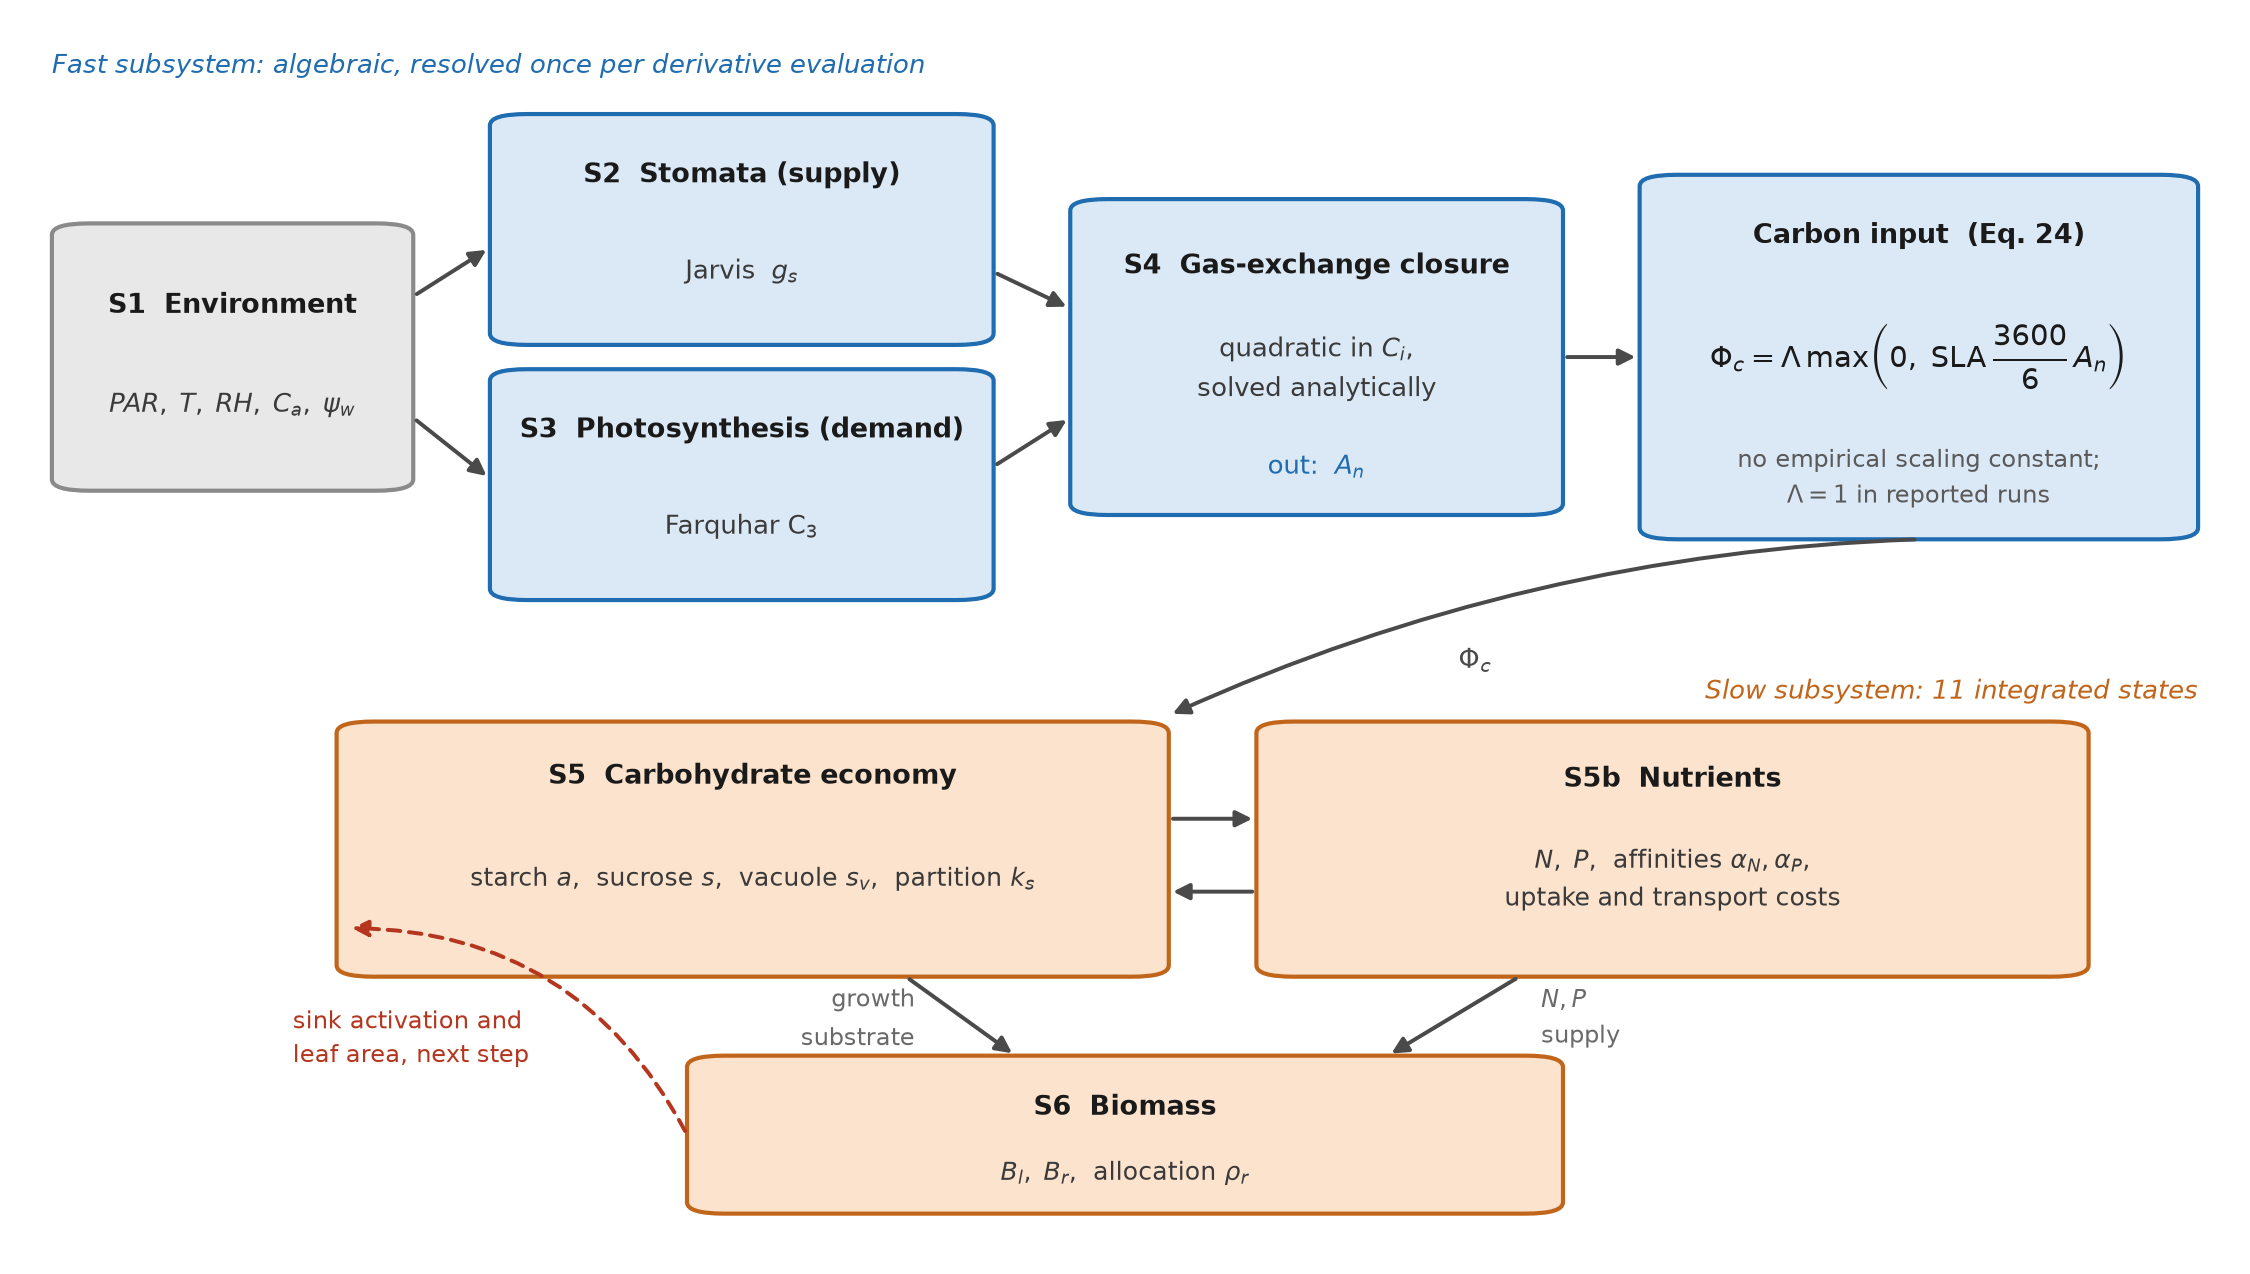
\includegraphics[width=\textwidth]{model_overview.png}
\caption{Model architecture and information flow through one derivative
evaluation. The fast subsystem (blue) is algebraic and is resolved once per
evaluation: environmental forcing S1 drives the stomatal supply function S2 and
the photosynthetic demand function S3, which are closed against each other in S4
as a quadratic in the intercellular CO$_2$ concentration and solved in closed
form. The resulting net assimilation is converted to the model carbon input
$\Phi_c$ by Eq.~\eqref{eq:conversion}, which the figure reproduces so that the
conversion can be read without turning back; there is no empirical scaling
constant in it. The slow subsystem (orange) comprises the eleven integrated states: the
carbohydrate economy S5, nutrient acquisition with its explicit costs S5b, and
leaf and root biomass S6. The dashed return arrow is the only slow-to-fast
signal in the architecture and it is narrow: leaf biomass enters the
gas-exchange layer solely as a viability gate, which returns zero assimilation
below $B_l = 0.001$~gFW and has no effect above it. Sink activation is a
feedback within the carbohydrate economy, driven by the sucrose pool and not by
biomass, so it is drawn inside S5. Arrows show the direction of information flow, not stoichiometric
mass transfer; the carbon budget is stated in
Section~\ref{sec:carbon_closure}.}
\label{fig:overview}
\end{figure*}

\subsection{Conceptual model and system decomposition}
\label{sec:conceptual}

The system is a single vegetative \textit{Arabidopsis} plant with its immediate
physical environment. Radiation, air temperature, humidity, ambient CO$_2$, leaf
water potential and soil nutrient concentrations cross the boundary as external
inputs. Carbon and nutrient acquisition, storage and allocation to leaf and root
biomass are internal states. The plant is two mass compartments, leaf and root,
without explicit geometry, so internal transport is described by aggregate
pools. This lumped decomposition and the carbon--nutrient allocation states
follow the whole-plant growth framework of \citet{Tedone2020}, whose prescribed
carbon input is here replaced by a computed gas-exchange layer.

Figure~\ref{fig:overview} shows the decomposition into six submodels and the
signals they exchange.
\begin{enumerate}\itemsep2pt
\item[\textbf{S1}] \emph{Environmental forcing} maps clock time to the light switch
      and the micro-climate. \emph{In:} $t$, scenario parameters. \emph{Out:}
      $\mathit{PAR}$, $T$, $\mathit{RH}$, $\mathit{VPD}$, $C_a$, $\psi_w$, $L$.
\item[\textbf{S2}] \emph{Stomatal conductance (supply)}, a multiplicative Jarvis
      model. \emph{In:} $\mathit{PAR}$, $\mathit{VPD}$, $T$, $C_a$, $\psi_w$.
      \emph{Out:} $g_s$.
\item[\textbf{S3}] \emph{Leaf photosynthesis (demand)}, the Farquhar C$_3$ model.
      \emph{In:} $\mathit{PAR}$, $C_i$, $V_{c\max}$, $J_{\max}$. \emph{Out:}
      $A_n(C_i)$.
\item[\textbf{S4}] \emph{Gas-exchange coupling} closes supply against demand.
      \emph{In:} $g_s$, $A_n(C_i)$, $C_a$. \emph{Out:} $A_n$, $C_i$.
\item[\textbf{S5}] \emph{Carbohydrate and nutrient economy} holds the diel starch
      and sucrose pools, the vacuolar compartment, and sucrose-limited N and P
      uptake with its costs. \emph{In:} $\Phi_c$, soil $N_s$, $P_s$. \emph{Out:}
      $s$, $U_N$, $U_P$.
\item[\textbf{S6}] \emph{Growth and allocation} converts exported sucrose into
      leaf and root biomass under functional-balance control. \emph{In:} $s$,
      $\alpha_N$, $\alpha_P$, $\varsigma$. \emph{Out:} $B_l$, $B_r$, $\rho_r$.
\end{enumerate}

Submodels S2--S4 form a fast algebraic subsystem. Leaf gas exchange equilibrates
within seconds, so it is treated as instantaneously relaxed relative to the slow
states in S5 and S6, which evolve over the diel cycle. It is therefore not
integrated but evaluated in closed form at every derivative call, as an
algebraic constitutive layer inside the derivative of the slow states
\citep{Cellier1991,Zeigler2000}. This separation organises both the formulation
and the implementation.

Only one signal returns from the slow subsystem to the fast one: leaf biomass
$B_l$ acts as a viability gate, and the carbon input is zero when
$B_l < B_{l,\min}$. The photosynthetic capacities $V_{c\max}$ and $J_{\max}$ are
fixed parameters and do not respond to nitrogen or carbohydrate status.
Figure~\ref{fig:overview} must therefore not be read as showing a capacity
feedback that the equations do not contain.

The formulation rests on six assumptions.
\begin{enumerate}\itemsep1pt
\item[(A1)] The plant is lumped into leaf and root compartments; no within-organ
      gradients or canopy architecture are resolved.
\item[(A2)] Leaf gas exchange is at steady state at every instant, so
      intercellular CO$_2$ is an algebraic balance and not a state.
\item[(A3)] Stomatal conductance responds multiplicatively to the environment and
      not to the assimilation rate \citep{Jarvis1976,Damour2010}.
\item[(A4)] Transitory starch is mobilised at a nocturnal rate paced by night
      length, as the observed near-linear depletion indicates
      \citep{Graf2010,Scialdone2013}.
\item[(A5)] Active nutrient uptake is limited by cytosolic sucrose, so carbon and
      nutrient acquisition are co-limiting \citep{Smith2007}.
\item[(A6)] Partitioning follows functional-balance theory: investment shifts
      towards the most limiting resource
      \citep{Thornley1972,ThornleyJohnson1990}.
\end{enumerate}

\subsection{State-space representation}
\label{sec:state}

The slow states form the vector $X(t)\in\mathbb{R}^{11}$ governed by

\begin{equation}
\frac{dX(t)}{dt} = f\!\left(X(t),\,U(t),\,\boldsymbol{\theta},\,t\right),
\label{eq:ode_general}
\end{equation}

where $U(t)$ is the exogenous forcing and $\boldsymbol{\theta}$ the time-invariant
parameter set. The explicit time dependence enters only through the diel forcing. In
the order used by the state packing routine of the implementation,

\begin{equation}
X(t) =
\left[
k_s,\; a,\; s,\; \alpha_N,\; \alpha_P,\; N,\; P,\; \rho_r,\; B_l,\; B_r,\; s_v
\right]^{\mathsf{T}}.
\label{eq:state_vector}
\end{equation}

Each symbol is defined in Table~\ref{tab:states}. Total biomass $B = B_l + B_r$ is
recomputed from the two biomass states whenever it is needed and is not integrated
as a twelfth state.

The pool states $a$, $s$, $s_v$, $N$ and $P$ are normalised model pools on a
nominal per-fresh-weight basis, not concentrations of a growing body. We adopt
this reading because it is the one under which the implemented balance equations
are exact: no growth-dilution term appears in Eqs.~\eqref{eq:starch},
\eqref{eq:sucrose}, \eqref{eq:sucrose_vac}, \eqref{eq:dN} or~\eqref{eq:dP}. The
cost is that $a$ and $s$ are not directly measured tissue concentrations, so the
carbohydrate comparison in Section~\ref{sec:results} is a comparison of shape and
timing after multiplicative alignment, not of absolute level.

The forcing vector is

\begin{equation}
U(t) =
\left[
\mathit{PAR}(t),\; T(t),\; \mathit{RH}(t),\; \mathit{VPD}(t),\; C_a,\;
\psi_w,\; L(t)
\right]^{\mathsf{T}},
\label{eq:input_vector}
\end{equation}

The deficit $\mathit{VPD}$ is a diagnostic function of $T$ and $\mathit{RH}$
through Eq.~\eqref{eq:vpd} and is not an independent input; it is listed because it
enters the stomatal response directly. In the scenarios reported here
$\mathit{RH}$, $C_a$ and $\psi_w$ are constant; $T$ is either constant or
thermoperiodic, and the chamber scenarios against which the model is evaluated
hold $21\,^{\circ}$C in the light and $19\,^{\circ}$C in darkness. The
time-varying inputs are therefore $\mathit{PAR}$, $L$ and, under the chamber
protocol, $T$.

\begin{table}[!htbp]
\centering
\small
\caption{State variables, environmental inputs and the principal derived
quantities. Pool states are normalised model pools on a nominal per-fresh-weight
basis (Section~\ref{sec:state}). ``Derived'' quantities are recomputed
algebraically at every derivative evaluation and are not integrated.}
\label{tab:states}
\begin{tabular}{@{}lllp{34mm}@{}}
\toprule
Symbol & Meaning & Unit & Role \\
\midrule
$k_s$        & Starch partition coefficient       & --                            & state, Eq.~\eqref{eq:dks} \\
$a$          & Transitory starch pool             & $\mu\mathrm{mol\,C_6\,gFW^{-1}}$ & state, Eq.~\eqref{eq:starch} \\
$s$          & Cytosolic sucrose pool             & $\mu\mathrm{mol\,C_6\,gFW^{-1}}$ & state, Eq.~\eqref{eq:sucrose} \\
$s_v$        & Vacuolar sucrose pool              & $\mu\mathrm{mol\,C_6\,gFW^{-1}}$ & state, Eq.~\eqref{eq:sucrose_vac} \\
$\alpha_N$   & Nitrogen investment state          & --                            & state, Eq.~\eqref{eq:dalphaN} \\
$\alpha_P$   & Phosphorus investment state        & --                            & state, Eq.~\eqref{eq:dalphaP} \\
$N$          & Internal nitrogen pool             & $\mu\mathrm{mol\,N\,gFW^{-1}}$ & state, Eq.~\eqref{eq:dN} \\
$P$          & Internal phosphorus pool           & $\mu\mathrm{mol\,P\,gFW^{-1}}$ & state, Eq.~\eqref{eq:dP} \\
$\rho_r$     & Sucrose-to-root allocation state   & --                            & state, Eq.~\eqref{eq:drhor} \\
$B_l$        & Leaf biomass                       & gFW                           & state, Eq.~\eqref{eq:dBl} \\
$B_r$        & Root biomass                       & gFW                           & state, Eq.~\eqref{eq:dBr} \\
\midrule
$\mathit{PAR}$ & Photosynthetically active radiation & $\mu\mathrm{mol\,m^{-2}\,s^{-1}}$ & input, Eq.~\eqref{eq:par_profile} \\
$L$          & Light/dark switch                  & --                            & input, Eq.~\eqref{eq:photoperiod} \\
$T$          & Leaf temperature                   & $^\circ$C                     & input, constant \\
$\mathit{RH}$& Relative humidity                  & \%                            & input, constant \\
$C_a$        & Ambient CO$_2$ concentration       & $\mu\mathrm{mol\,mol^{-1}}$   & input, constant \\
$\psi_w$     & Leaf water potential               & MPa                           & input, constant \\
$N_s,P_s$    & Soil N, P concentration            & $\mu\mathrm{mol\,cm^{-3}}$    & input, constant \\
\midrule
$\mathit{VPD}$ & Vapour pressure deficit          & kPa                           & derived, Eq.~\eqref{eq:vpd} \\
$g_s,g_c$    & Conductance to H$_2$O, to CO$_2$   & $\mathrm{mol\,m^{-2}\,s^{-1}}$& derived, Eqs.~\eqref{eq:jarvis}, \eqref{eq:supply} \\
$C_i$        & Intercellular CO$_2$ concentration & $\mu\mathrm{mol\,mol^{-1}}$   & derived, Eq.~\eqref{eq:ci_root} \\
$A_c,A_j$    & Rubisco-, RuBP-limited rate        & $\mu\mathrm{mol\,m^{-2}\,s^{-1}}$ & derived, Eqs.~\eqref{eq:Ac}, \eqref{eq:Aj} \\
$A_n$        & Net leaf assimilation              & $\mu\mathrm{mol\,m^{-2}\,s^{-1}}$ & derived, Eq.~\eqref{eq:An} \\
$J$          & Electron transport rate            & $\mu\mathrm{mol\,m^{-2}\,s^{-1}}$ & derived, Eq.~\eqref{eq:J_root} \\
$\Phi_c$     & Carbon input to the pools          & $\mu\mathrm{mol\,C_6\,gFW^{-1}\,h^{-1}}$ & derived, Eq.~\eqref{eq:conversion} \\
$D_a$        & Starch degradation flux            & $\mu\mathrm{mol\,C_6\,gFW^{-1}\,h^{-1}}$ & derived, Eq.~\eqref{eq:starch_degradation} \\
$E$          & Exportable sucrose term            & $\mu\mathrm{mol\,C_6\,gFW^{-1}}$ & derived, Eq.~\eqref{eq:export} \\
$U_N,U_P$    & Realised N, P uptake               & $\mu\mathrm{mol\,gFW^{-1}\,h^{-1}}$ & derived, Eq.~\eqref{eq:uptake} \\
$\varsigma$  & Stoichiometric signal              & --                            & derived, Eq.~\eqref{eq:stoich} \\
$B$          & Total biomass, $B_l+B_r$           & gFW                           & derived \\
\bottomrule
\end{tabular}
\end{table}

\subsection{Submodel S1: environmental forcing}
\label{sec:forcing}

Let $h(t) = t \bmod 24$ be the hour of day and $f$ the photoperiod length in
hours. The light switch is

\begin{equation}
L(t) =
\begin{cases}
1, & 0 \leq h(t) < f, \\
0, & f \leq h(t) < 24 ,
\end{cases}
\label{eq:photoperiod}
\end{equation}

and the incident radiation follows one of two daytime profiles, selected by
scenario:

\begin{equation}
\mathit{PAR}(t) =
\begin{cases}
\mathit{PAR}_{\max}, & \text{square wave},\; L=1, \\[4pt]
\mathit{PAR}_{\max}\,\sin\!\left(\pi\,h(t)/f\right), & \text{half sine},\; L=1, \\[4pt]
0, & L=0 .
\end{cases}
\label{eq:par_profile}
\end{equation}

The square wave represents a growth chamber, which delivers constant irradiance
over the light period; the half sine is a smooth idealisation of a natural light
course. The choice sets the daily light integral: the square wave gives
$\mathit{PAR}_{\max} f$ and the half sine $(2/\pi)\,\mathit{PAR}_{\max} f$. A run
matching a chamber experiment must therefore use the square profile at the
chamber irradiance. One consequence of the design affects every photoperiod
result. With $\mathit{PAR}_{\max}$ held fixed, changing the photoperiod changes
the daily light integral in proportion. Day length and daily photon dose are
confounded by construction, so a photoperiod response in this model is a joint
response to duration and dose.

The vapour pressure deficit is obtained from leaf temperature and relative
humidity through the Tetens relation \citep{Monteith1965,Nobel2009},

\begin{equation}
\mathit{VPD} = e_s\left(1 - \frac{\mathit{RH}}{100}\right),
\qquad
e_s = 0.61078\,\exp\!\left(\frac{17.27\,T}{T + 237.3}\right),
\label{eq:vpd}
\end{equation}

with $e_s$ and $\mathit{VPD}$ in kPa and $T$ in $^\circ$C. Where a
thermoperiod is specified, $T$ takes its day value while $L=1$ and its night
value while $L=0$; otherwise $T$ is constant.

\subsection{Submodel S2: stomatal conductance (supply)}
\label{sec:jarvis}

This submodel returns the stomatal conductance and forms the supply side of gas
exchange. It carries no dependence on the assimilation rate (A3). Conductance
is a maximal value reduced by a product of dimensionless environmental
modifiers, each bounded in $[0,1]$ \citep{Jarvis1976,Damour2010}:

\begin{equation}
g_s = g_{s,\max}\;
f_{\mathit{PAR}}(\mathit{PAR})\;
f_{\mathit{VPD}}(\mathit{VPD})\;
f_T(T)\;
f_{\mathit{CO_2}}(C_a)\;
f_w(\psi_w).
\label{eq:jarvis}
\end{equation}

The multiplicative closure assumes that the environmental controls act
independently. It is a widely used empirical conductance model and needs no
optimisation step at runtime \citep{Damour2010,Buckley2017}. The maximal
conductance $g_{s,\max}$ is a separate parameter from the shape parameters of the
modifiers. Each modifier can then be required to equal unity at its own
non-limiting reference condition, so changing the shape of one modifier does not
rescale the whole conductance.

The light response is a saturating hyperbola with a residual conductance
$b_{10}$ below a breakpoint $q = b_{10}/b_1$,

\begin{equation}
f_{\mathit{PAR}} =
\begin{cases}
b_{10}, & \mathit{PAR} \leq q, \\[6pt]
\dfrac{b_1 b_2\,(\mathit{PAR}-q)}{b_1 + b_2\,(\mathit{PAR}-q)}, & \mathit{PAR} > q .
\end{cases}
\label{eq:jarvis_par}
\end{equation}

The response to atmospheric demand is linear and floored at zero, and the
response to leaf water potential is a saturating recovery above a closure
potential $\psi_{\min}$, clipped to $[0,1]$:

\begin{align}
f_{\mathit{VPD}} &= \max\!\left(0,\; 1 - b_5\,\mathit{VPD}\right),
\label{eq:jarvis_vpd}\\[4pt]
f_w &= 1 - \exp\!\left(-b_6\,(\psi_w - \psi_{\min})\right).
\label{eq:jarvis_water}
\end{align}

The temperature response is a skewed optimum with zeros at $T_1$ and $T_h$,

\begin{equation}
f_T =
\begin{cases}
b_3\,(T - T_1)\,(T_h - T)^{b_4}, & T_1 < T < T_h, \\[4pt]
0, & \text{otherwise},
\end{cases}
\qquad
b_4 = \frac{T_h - T_0}{T_0 - T_1},
\quad
b_3 = \frac{1}{(T_0 - T_1)(T_h - T_0)^{b_4}} .
\label{eq:jarvis_T}
\end{equation}

The two constants $b_3$ and $b_4$ are not free. They are fixed by requiring
stationarity at $T_0$ and $f_T(T_0)=1$, which places the maximum at $T_0$ and
normalises the modifier to unity there. With $T_1 = 5$, $T_0 = 25$ and
$T_h = 45\,^\circ$C this gives $b_4 = 1$, so the curve is a single-peaked
parabola and no clipping from above is needed.

The CO$_2$ response is piecewise linear in $C_a$, expressed in
$\mu\mathrm{mol\,mol^{-1}}$. It is constant below $100$, falls linearly to a floor
$b_8$ at $1000$, and equals that floor above it:

\begin{equation}
f_{\mathit{CO_2}} =
\begin{cases}
1, & C_a < 100, \\[4pt]
1 - b_7\,(C_a - 100), & 100 \leq C_a < 1000, \\[4pt]
b_8, & C_a \geq 1000,
\end{cases}
\qquad
b_7 = \frac{1 - b_8}{900} .
\label{eq:jarvis_co2}
\end{equation}

\subsection{Submodel S3: leaf photosynthesis (demand)}
\label{sec:farquhar}

This submodel returns net assimilation as a function of the intercellular
CO$_2$ concentration and forms the demand side of gas exchange. It is the
Farquhar--von~Caemmerer--Berry C$_3$ model, in which gross assimilation is the
smaller of a Rubisco-limited and an electron-transport-limited rate
\citep{Farquhar1980,vonCaemmerer2000}. The Rubisco-limited rate is

\begin{equation}
A_c = V_{c\max}\,
\frac{C_i - \Gamma^{*}}{C_i + K_c\!\left(1 + O/K_o\right)},
\label{eq:Ac}
\end{equation}

with $\Gamma^{*}$ the CO$_2$ compensation point in the absence of dark
respiration, $K_c$ and $K_o$ the Michaelis constants of Rubisco for CO$_2$ and
O$_2$, and $O$ the oxygen concentration. The electron-transport-limited rate is

\begin{equation}
A_j = J\,\frac{C_i - \Gamma^{*}}{4.5\,C_i + 10.5\,\Gamma^{*}},
\label{eq:Aj}
\end{equation}

where the denominator coefficients $4.5$ and $10.5$ encode the electron
requirement per carboxylation and per oxygenation under the standard
stoichiometry of RuBP regeneration
\citep{vonCaemmerer1981,vonCaemmerer2000}. Net assimilation is the limiting
rate less dark respiration,

\begin{equation}
A_n = \min(A_c,\,A_j) - R_d .
\label{eq:An}
\end{equation}

The electron transport rate follows from $\mathit{PAR}$ through the
non-rectangular hyperbola
$\theta J^2 - (J_{\max} + \phi\,\mathit{PAR})J + J_{\max}\phi\,\mathit{PAR} = 0$
\citep{Farquhar1980,Farquhar1984}, of which the lower root is taken,

\begin{equation}
J = \frac{\left(J_{\max}+\phi\,\mathit{PAR}\right)
- \sqrt{\left(J_{\max}+\phi\,\mathit{PAR}\right)^{2}
- 4\,\theta\,J_{\max}\,\phi\,\mathit{PAR}}}{2\,\theta},
\label{eq:J_root}
\end{equation}

with $\phi$ the apparent quantum yield for electron transport and $\theta$ the
curvature of the light response.

No irradiance threshold is applied to this submodel: the carbon input is evaluated
whenever $\mathit{PAR} > 0$ and $B_l \geq B_{l,\min}$. A threshold is unnecessary
because, with the closed-form operating point of Section~\ref{sec:closure}, the net
rate passes continuously through zero at the light compensation point and the clamp
in Eq.~\eqref{eq:conversion} returns exactly zero below it. Below that point $A_n$
itself remains negative. It is the carbon input that is clamped and not $A_n$, so
respiratory efflux is never counted as an assimilatory gain.

\subsection{Submodel S4: gas-exchange coupling}
\label{sec:closure}

Equations~\eqref{eq:Ac}--\eqref{eq:An} give demand as a function of a
concentration that is itself set by supply. Fickian diffusion of CO$_2$ through
the stomata gives

\begin{equation}
A_n = g_c\,(C_a - C_i),
\qquad
g_c = \frac{g_s}{1.6},
\label{eq:supply}
\end{equation}

where the factor $1.6$ converts the conductance to water vapour into a conductance
to CO$_2$, which diffuses more slowly in air \citep{vonCaemmerer2000,Nobel2009}.
Because $A_n$ depends on $C_i$ and $C_i$ depends on $A_n$, the operating point is
the mutual solution of Eqs.~\eqref{eq:An} and~\eqref{eq:supply}. How that coupling
is solved is the main methodological choice in the formulation.

The system needs no iteration. Both Farquhar branches have the same rational form
in $C_i$,

\begin{equation}
A = \frac{\mathrm{num}\,(C_i - \Gamma^{*})}{d_1 C_i + d_0} - R_d,
\qquad
(\mathrm{num},\,d_1,\,d_0) =
\begin{cases}
\bigl(V_{c\max},\; 1,\; K_c(1 + O/K_o)\bigr), & \text{Rubisco branch}, \\[4pt]
\bigl(J,\; 4.5,\; 10.5\,\Gamma^{*}\bigr), & \text{transport branch},
\end{cases}
\label{eq:branch_form}
\end{equation}

so the branch coefficients are read directly off Eqs.~\eqref{eq:Ac}
and~\eqref{eq:Aj} without dividing through. Equating supply and demand,

\begin{equation}
g_c\,(C_a - C_i)\,(d_1 C_i + d_0)
= \mathrm{num}\,(C_i - \Gamma^{*}) - R_d\,(d_1 C_i + d_0),
\label{eq:closure_raw}
\end{equation}

and clearing the denominator gives a quadratic in $C_i$,

\begin{equation}
a\,C_i^{2} + b\,C_i + c = 0,
\qquad
\begin{aligned}
a &= -g_c\,d_1, \\
b &= g_c\,(d_1 C_a - d_0) - \mathrm{num} + R_d\,d_1, \\
c &= g_c\,d_0\,C_a + \mathrm{num}\,\Gamma^{*} + R_d\,d_0 .
\end{aligned}
\label{eq:ci_quadratic}
\end{equation}

Exactly one root of Eq.~\eqref{eq:ci_quadratic} is admissible on each branch, and
no search is needed to identify it. The admissibility condition is $C_i \geq 0$
alone. For $g_c > 0$ the leading coefficient is $a = -g_c d_1 < 0$, while $c > 0$
because every factor in it is positive. The product of the roots $c/a$ is
therefore negative, so each branch has one positive and one negative root, and the
positive one is the operating point:

\begin{equation}
C_i =
\frac{-b - \sqrt{b^{2} - 4ac}}{2a}
\;>\; 0 .
\label{eq:ci_root}
\end{equation}

Substituting this root back into Eq.~\eqref{eq:branch_form} gives the branch
assimilation, and the smaller of the two branch values is returned. That is the
same co-limitation rule as $\min(A_c,A_j)$ in Eq.~\eqref{eq:An}, applied after
each branch has been closed against supply rather than before. Because exactly one
root per branch is admissible, the minimum over the two branches is the solution
of the coupled system and not merely a candidate for it.

The admissibility rule deserves emphasis, because the natural guess is wrong. No
upper bound on $C_i$ is imposed, and a root above the ambient concentration is
retained rather than rejected. By Eq.~\eqref{eq:supply}, $C_i > C_a$ is exactly
what the supply relation returns whenever $A_n < 0$, that is, whenever the leaf is
a net source and CO$_2$ diffuses outward. The condition $0 \le C_i \le C_a$ is
therefore not a physical constraint here, and imposing it would discard the
correct root twice a day.

The vanishing-conductance case has a physical answer rather than a clamp, and the
one-sided limit and the closed boundary are two different states. As
$g_c \to 0^{+}$ the quadratic degenerates: $a \to 0$ and
$b \to R_d d_1 - \mathrm{num}$, and the finite root of the remaining linear
equation is

\begin{equation}
\lim_{g_c \to 0^{+}} C_i
= \frac{\mathrm{num}\,\Gamma^{*} + R_d d_0}{\mathrm{num} - R_d d_1},
\label{eq:ci_limit}
\end{equation}

provided the denominator is positive, which holds for both branches at the
parameter values used here. Substituting this root into
Eq.~\eqref{eq:branch_form} gives $A_b = R_d$ and hence $A_n \to 0$: supply and
demand meet at the compensation point, where diffusion delivers nothing and
gross assimilation exactly pays respiration. The limit is a finite
$C_i$, not $\Gamma^{*}$. At the production values it evaluates to
$67.94~\mu\mathrm{mol\,mol^{-1}}$ on the Rubisco-limited branch and
$53.35$ on the electron-transport-limited branch, and a numerical sweep in
$g_c$ reproduces both.

Exactly closed stomata are a separate case. At $g_c = 0$ the supply relation
carries no information about $C_i$, the quadratic is empty, and the physical
state is a leaf that admits no CO$_2$ and only respires. The implementation
returns that state directly at the boundary $g_c \leq 0$,

\begin{equation}
C_i = \Gamma^{*}, \qquad A_n = -R_d ,
\label{eq:ci_dark}
\end{equation}

which is the dark limit and replaces a clamp on the conductance.

This assignment is an implementation boundary convention and not the continuous
extension of Eq.~\eqref{eq:ci_limit}. The one-sided limit derived above gives
$A_n \to 0$ as $g_c \to 0^{+}$, whereas the convention returns $A_n = -R_d$ at
$g_c = 0$, so the two differ by $R_d$ at the boundary. We state the difference
rather than smooth it over. The convention is the physically meaningful one for a
leaf with no gas exchange, since gross assimilation requires a CO$_2$ supply that
a shut stoma does not provide, while the limit describes a leaf whose stomata are
almost shut and which is still exchanging enough CO$_2$ to break even. Whether
the discrepancy matters is a question about the trajectory: the conductance model
of Section~\ref{sec:jarvis} has a positive floor on its light response, so
$g_c = 0$ is never reached in any reported run and the branch is not exercised.
Respiration in darkness is carried by the same expression that carries
assimilation in the light.

One numerical caveat belongs with this derivation. Written in the form above the
quadratic loses significance when $a = -g_c d_1$ becomes comparable to the
rounding error of $b$, which at these parameter values occurs below
$g_c \approx 10^{-8}$; a sweep to $g_c = 10^{-11}$ returns a spurious positive
$A_n$. The conductance model of Section~\ref{sec:jarvis} has a positive floor on
its light response, so no reported run enters that range, and we record the
bound rather than rely on it being unreachable.

Two properties of this closure matter for the rest of the paper. The branch-wise
quadratic is solved once per derivative evaluation, with no inner iteration in the
production configuration, so the derivative is a deterministic function of $(X,t)$
as an embedded-pair error estimate assumes. And the solution is exact up to
floating-point arithmetic, so no inner convergence tolerance interacts with the
outer error control. Section~\ref{sec:implementation} reports the substitution
residual that verifies this.

\subsection{From assimilation to model carbon input}
\label{sec:conversion}

The leaf-level net assimilation $A_n$
($\mu\mathrm{mol\,CO_2\,m^{-2}\,s^{-1}}$) must be converted to the carbon
input $\Phi_c$ that drives the carbohydrate pools
($\mu\mathrm{mol\,C_6\,gFW^{-1}\,h^{-1}}$). The conversion is

\begin{equation}
\Phi_c = \Lambda\;\max\!\left(0,\;
\underbrace{\mathrm{SLA}}_{\mathrm{m^2\,gFW^{-1}}}\;
\underbrace{\frac{3600}{6}}_{\mathrm{s\,h^{-1}\ /\ mol\,CO_2\,per\,mol\,C_6}}\;
A_n \right),
\qquad L = 1 ,
\label{eq:conversion}
\end{equation}

and $\Phi_c = 0$ when $L = 0$ or $B_l < B_{l,\min}$. Three factors carry the whole
unit conversion and none of them is free: $\mathrm{SLA}$ moves the flux to a
per-fresh-weight basis, the factor $3600$ converts seconds to hours, and the
divisor $6$ converts moles of CO$_2$ to moles of hexose. Their product is
$600\,\mathrm{SLA}$, so at the measured $\mathrm{SLA}$ of Table~\ref{tab:params}
the coefficient is fixed by the units and no empirical scaling constant enters the
carbon-input pathway. The clamp keeps a negative $A_n$ out of the pools, as
discussed in Section~\ref{sec:farquhar}.

The factor $\Lambda$ is a sink-limitation term that down-regulates assimilation
as the starch pool fills,

\begin{equation}
\Lambda = \min\!\left(1,\; \max\!\left(\lambda_c,\;
\lambda_c + (1-\lambda_c)\,\frac{a_{\max} - a}{a_{\max}}\right)\right),
\qquad
a_{\max} = D_{a,\max}\,(24 - f),
\label{eq:feedback}
\end{equation}

where $\lambda_c$ is the residual assimilation fraction at a full pool and the
ceiling $a_{\max}$ scales with night length, since a longer night requires a
larger reserve. The inner $\max$ bounds the term at its value at the ceiling, so a
pool above $a_{\max}$ cannot drive $\Lambda$ negative and reverse the sign of
assimilation. In all reported runs $\lambda_c = 1$, which makes $\Lambda = 1$
identically and the sink limitation inactive. The equation is given because the
term is present in the right-hand side and is used in the ablation of
Section~\ref{sec:protocol}; its shipped value is stated so that a reader knows
the reported results do not depend on it.

\subsection{Submodel S5: carbohydrate economy}
\label{sec:carbohydrates}

The carbon input $\Phi_c$ is split between transitory starch and cytosolic sucrose
by the partition coefficient $k_s$. This coefficient is a state with its own
dynamics rather than a fixed split, so the plant can shift it during the day and
again at night in response to the sucrose level. The diel carbohydrate balance is
then an emergent property of the model and not a prescribed schedule
\citep{Stitt2012,Mengin2017}.

\paragraph{Starch partition.}
Let $\sigma^{-} = s_{\min}/(s_{\min}+s)$ and
$\sigma^{+} = s/(s+s_{\max})$ be the sucrose-deficit and sucrose-excess
fractions, both in $[0,1]$ and both saturating. The partition state follows

\begin{equation}
\frac{dk_s}{dt}
= \underbrace{L\left[
-\,k_s\,\lambda_{sdr}\,\sigma^{-}
+\left(1-k_s\right)\lambda_{sdi}\,\sigma^{+}
\right]}_{\text{light phase}}
+\underbrace{\left(1-L\right)\left(1-k_s\right)\lambda_{sni}\,\sigma^{-}}_{\text{dark phase}} .
\label{eq:dks}
\end{equation}

Each term has a direct interpretation. In the light, a low sucrose level makes
$\sigma^{-}$ large and the first term reduces $k_s$, so more incoming carbon goes
to sucrose and the immediate demand is met. A high sucrose level makes
$\sigma^{+}$ large and the second term raises $k_s$, so surplus carbon is stored
as starch. In the dark there is no input to partition, and the third term raises
$k_s$ when sucrose is low, returning the state to a storage-biased value before
the next light period. The factors $k_s$ and $(1-k_s)$ keep the state in $[0,1]$
without a clamp, since each term vanishes at the bound it approaches. The three
rate coefficients set the speed of the day-reduction, day-increase and
night-increase responses.

\paragraph{Starch pool.}
Starch gains the partitioned share of the input and loses the nocturnal
degradation flux $D_a$,

\begin{equation}
\frac{da}{dt} = k_s\,\Phi_c - D_a .
\label{eq:starch}
\end{equation}

The degradation flux implements the observed pacing of starch mobilisation
against the remaining night length \citep{Graf2010,Scialdone2013}. Let
$a_{\mathrm{dusk}}$ be the starch content recorded at the last transition to
darkness and $a_{\min}$ the residual pool that is not mobilised. Then

\begin{equation}
D_a =
\left(1-L\right)
\min\!\left(
D_{a,\max},\;
\left[
\frac{h}{24} + \left(1-\frac{h}{24}\right)\left(1-\frac{s}{s+s_{\max}}\right)
\right]
\frac{a_{\mathrm{dusk}} - a_{\min}}{24 - f}
\right),
\label{eq:starch_degradation}
\end{equation}

and $D_a = 0$ if $a_{\mathrm{dusk}} < a_{\min}$. The quotient
$(a_{\mathrm{dusk}}-a_{\min})/(24-f)$ is the constant rate that would exactly
exhaust the mobilisable reserve over the night, which is the rate the
measurements show. The bracketed factor modulates it: when sucrose is abundant
the second summand is small and degradation is slowed, so the reserve is spared.
The outer $\min$ bounds the flux by the degradation capacity $D_{a,\max}$ and the
factor $(1-L)$ confines it to darkness. Two properties matter for the limitation
reported in Section~\ref{sec:limitations}. The reference level
$a_{\mathrm{dusk}}$ is sampled at dusk and held over the night, so it is not a
continuous function of the state, and the divisor $24-f$ is the nominal rather
than the remaining night length.

\paragraph{Sucrose pools.}
Cytosolic sucrose receives the unpartitioned share of the input and the starch
degradation flux, and pays four costs: nutrient uptake, phloem transport,
maintenance respiration, and export to the sinks. It also exchanges with the
vacuolar pool. The balance is

\begin{equation}
\frac{ds}{dt}
= \left(1-k_s\right)\Phi_c
+ D_a
- C_u
- C_t
- R_m
- \eta\,E
- k_{\mathrm{in}}\,s
+ k_{\mathrm{out}}\,s_v
- C_g ,
\label{eq:sucrose}
\end{equation}

\begin{equation}
\frac{ds_v}{dt} = k_{\mathrm{in}}\,s - k_{\mathrm{out}}\,s_v .
\label{eq:sucrose_vac}
\end{equation}

The vacuolar compartment is a passive first-order buffer with influx rate
$k_{\mathrm{in}}$ and efflux rate $k_{\mathrm{out}}$, and the two rate constants
appear with opposite signs in Eqs.~\eqref{eq:sucrose} and~\eqref{eq:sucrose_vac},
so the exchange conserves sucrose. It represents the measured separation of leaf
sucrose into an active cytosolic fraction and a larger stored vacuolar fraction
\citep{Lohaus2000,Nadwodnik2008}. Only $s$ enters the cost and export terms, so
the buffer damps the diel excursion of the active pool without adding or removing
carbon, with relaxation time $1/(k_{\mathrm{in}}+k_{\mathrm{out}})$.

The export term is the phloem-loading flux, and it carries the sugar-induced
sink activation:

\begin{equation}
E =
\underbrace{\min\!\left(s,\;s_{\max}\right)}_{\text{loadable pool}}
\underbrace{\left[1 + \left(\frac{s}{K_s}\right)^{n_H}\right]}_{\text{sink activation}}
\underbrace{\left[\lambda_g + \left(1-\lambda_g\right)\left(1 - L + L\left(1-k_s\right)\right)\right]}_{\text{loading efficiency}} .
\label{eq:export}
\end{equation}

The activation factor multiplies the loadable pool before the loading efficiency
is applied, so it scales the export flux and not the pool size. Its form requires
comment because it is not the bounded Hill function. A saturating factor
$s^{n_H}/(K_s^{n_H}+s^{n_H})$ is bounded above by one and can therefore only
weaken the drain, which is the wrong direction. Sucrose induces its own
consumption, by raising invertase activity and sink-tissue transporter
expression, so consumption capacity rises with the pool
\citep{Smith2007,Stitt2012}. The unbounded factor $1+(s/K_s)^{n_H}$ represents
this: it is close to one at $s \ll K_s$, and at $s \gg K_s$ the drain scales as
$s^{1+n_H}$. The steady-state pool then grows as the $1/(1+n_H)$ power of the
supply, so the sucrose level is held near $K_s$ while assimilation varies. A
first-order drain with constant coefficients cannot hold a level in this way. The
half-activation constant $K_s$ is one of the four calibrated parameters
(Table~\ref{tab:fitted}).

The loading efficiency term interpolates between a floor $\lambda_g$ and unity.
It equals one at night and $\lambda_g + (1-\lambda_g)(1-k_s)$ in the light, so
export is least efficient when the light-phase partition is strongly biased to
starch. The remaining costs are

\begin{align}
C_u &= c_N\,U_N + c_P\,U_P ,
\label{eq:uptake_cost}\\[3pt]
C_t &= \tau_c\left(r_m\,s + \eta\,E\right),
\label{eq:transport_cost}\\[3pt]
R_m &= r_m\,s ,
\label{eq:respiration}\\[3pt]
C_g &=
\begin{cases}
Y\left(\dfrac{dB_l}{dt} + \dfrac{dB_r}{dt}\right), &
\dfrac{dB_l}{dt} + \dfrac{dB_r}{dt} > 0, \\[10pt]
0, & \text{otherwise} .
\end{cases}
\label{eq:growth_cost}
\end{align}

The uptake cost $C_u$ prices the realised nutrient fluxes at the sucrose
consumption coefficients $c_N$ and $c_P$, and is evaluated after
Eq.~\eqref{eq:uptake} so that it uses the fluxes of the current state. The
transport cost $C_t$ is a fixed fraction $\tau_c$ of the respiratory and loading
fluxes. Maintenance respiration $R_m$ is first order in the cytosolic pool with
specific rate $r_m$, charged over all hours as in the source formulation
\citep{Tedone2020}. The construction cost $C_g$ prices the biomass actually
built, at $Y$ moles of hexose per gram of fresh biomass. It is applied after both
growth rates have been evaluated and is one-sided: senescence returns tissue but
does not refund construction carbon.

The term is present in the formulation but inactive in the results. Every run
reported in this paper uses $Y = 0$, which is the value carried by both the
shipped configuration and the compiled default, so no carbon is charged for the
biomass that is built. The growth law of Eq.~\eqref{eq:dBl} therefore converts
sucrose to biomass without paying a stoichiometric price, and the coefficient
$\lambda_{sb}$ absorbs that conversion empirically. Two consequences follow and
we state them here rather than leave them implicit. The carbon budget of
Section~\ref{sec:carbon_closure} is a bookkeeping statement about the
carbohydrate pools and not a whole-plant carbon balance, and the growth
coefficient calibrated in Section~\ref{sec:results:rgr} is a rate constant, not
a measured yield. The term is dormant and outside the formulation that this paper
evaluates, and activating it is not a matter of substituting a literature value.
Eq.~\eqref{eq:growth_cost} multiplies $Y$, in $\mu\mathrm{mol\,C_6\,gFW^{-1}}$,
by a biomass rate in $\mathrm{gFW\,h^{-1}}$, giving
$\mu\mathrm{mol\,C_6\,h^{-1}}$, while every other term of the sucrose equation
is written on the nominal per-fresh-weight basis of
Section~\ref{sec:state}. The two bases would have to be reconciled before
a sourced $Y$ could be switched on, and the reconciliation would change the
calibration. We record the mismatch here rather than present activation as a
substitution.

\subsection{Submodel S5b: nutrient uptake and costs}
\label{sec:nutrients}

Nutrient acquisition is active and therefore carbon-limited (A5). It is
represented in three stages: a soil-availability rate, an allocation of root
capacity, and a sucrose-limited realisation.

The soil stage is Michaelis--Menten in the external concentration
\citep{Epstein1952,Tinker2000},

\begin{equation}
I_N = I_{N,\max}\,\frac{N_s}{N_s + K_N},
\qquad
I_P = I_{P,\max}\,\frac{P_s}{P_s + K_P} .
\label{eq:soil_uptake}
\end{equation}

The potential uptake scales this by the investment state and by the root
fraction of total biomass, and the realised uptake applies a sucrose limitation:

\begin{align}
\widehat{U}_N &= I_N\,\alpha_N\,\frac{B_r}{B + \varepsilon},
&
U_N &= \widehat{U}_N\,
\frac{s}{s + c_N\,\widehat{U}_N\,\tau + \varepsilon},
\label{eq:uptake}\\[3pt]
\widehat{U}_P &= I_P\,\alpha_P\,\frac{B_r}{B + \varepsilon},
&
U_P &= \widehat{U}_P\,
\frac{s}{s + c_P\,\widehat{U}_P\,\tau + \varepsilon} .
\notag
\end{align}

The saturating factor in Eq.~\eqref{eq:uptake} has a clear reading. The quantity
$c_N \widehat{U}_N \tau$ is the sucrose that the potential uptake would consume
over a reference interval $\tau = 1\,\mathrm{h}$, so it is a sucrose amount and
comparable with $s$. When the pool greatly exceeds it the factor approaches one and
uptake proceeds at its potential rate; when carbon is short the factor falls and
uptake is throttled. The constant $\varepsilon$ is the machine epsilon of the
working precision, guards the denominators only, and is not a model parameter.

The internal pools are balanced against two demands, structural and
photosynthetic:

\begin{align}
\frac{dN}{dt} &= U_N
- \left[r_m\left(s+a\right) + \eta\,E\right] r_{A,N}\,\frac{B_l}{B+\varepsilon}
- \frac{\Phi_c}{\Phi_{c,\max}}\,N_{ph}\,\nu ,
\label{eq:dN}\\[3pt]
\frac{dP}{dt} &= U_P
- \left[r_m\left(s+a\right) + \eta\,E\right] r_{A,P}\,\frac{B_l}{B+\varepsilon}
- \frac{\Phi_c}{\Phi_{c,\max}}\,P_{ph}\,\nu .
\label{eq:dP}
\end{align}

The first loss term charges nutrients against the carbon turnover of the shoot, at
the assimilation cost coefficients $r_{A,N}$ and $r_{A,P}$ and in proportion to
the leaf share of biomass. The second charges the nutrient requirement of
photosynthesis, scaled by the relative assimilation rate $\Phi_c/\Phi_{c,\max}$
and the conversion parameter $\nu$, with $N_{ph}$ and $P_{ph}$ the contents below
which assimilation would be nutrient limited. Those thresholds appear in the
saturation functions

\begin{equation}
\varphi_N = \max\!\left(0,\; \frac{2N}{N+N_{ph}} - 1\right),
\qquad
\varphi_P = \max\!\left(0,\; \frac{2P}{P+P_{ph}} - 1\right),
\label{eq:nutrient_saturation}
\end{equation}

which are zero at the threshold and approach one at large content.

These two functions are the only place where nutrient status could reach carbon
acquisition, and in the configuration reported here they do not reach it. They
enter the prescribed-input variant M0 of Section~\ref{sec:results:ablation}
through a multiplicative factor $\min(\varphi_N,\varphi_P)$ on the assimilation
rate. The Farquhar routine used for every reported result contains no nutrient
term, so under M1 and M2 assimilation is independent of $N$ and $P$, and the
coupling from nutrients to growth runs through the sucrose economy alone. The
architecture of Figure~\ref{fig:overview} shows no arrow from the nutrient
states to the gas-exchange layer for this reason.

The investment states $\alpha_N$ and $\alpha_P$ carry the acclimation of uptake
capacity. Each follows a two-term law. The first term drives investment up when the
nutrient is scarce or assimilation is high. The second drives it down when the pool
is full, or when the carbon price of uptake is high relative to the available
sucrose flux:

\begin{equation}
\frac{d\alpha_N}{dt}
= \left(1-\alpha_N\right)
\left[
\left(1 - \frac{U_N}{U_N + C_N + \varepsilon}\right)
\frac{N_{\max}}{N + N_{\max}}
+ \frac{\Phi_c}{\Phi_{c,\max}}
- \Omega
\right]
- \alpha_N
\left[
\frac{N}{N+N_{\min}}
+ \frac{c_N U_N}{c_N U_N + \Phi_c\left(1-k_s\right) + D_a + \varepsilon}
\right],
\label{eq:dalphaN}
\end{equation}

\begin{equation}
\frac{d\alpha_P}{dt}
= \left(1-\alpha_P\right)
\left[
\left(1 - \frac{U_P}{U_P + C_P + \varepsilon}\right)
\frac{P_{\max}}{P + P_{\max}}
+ \frac{\Phi_c}{\Phi_{c,\max}}
+ \Omega
\right]
- \alpha_P
\left[
\frac{P}{P+P_{\min}}
+ \frac{c_P U_P}{c_P U_P + \Phi_c\left(1-k_s\right) + D_a + \varepsilon}
\right],
\label{eq:dalphaP}
\end{equation}

where $C_N$ and $C_P$ are the nutrient cost terms and $\Omega$ is the
stoichiometric imbalance signal

\begin{equation}
\Omega = \alpha\,\lambda_k\,\frac{N - \omega P}{N + \omega P + \varepsilon},
\label{eq:imbalance}
\end{equation}

with $\alpha$ the corresponding investment state, $\omega$ the optimal N:P ratio
and $\lambda_k$ the gain. The sign of $\Omega$ is opposite in the two equations,
which is the coupling that makes the pair competitive: an excess of nitrogen
relative to the optimal ratio suppresses further nitrogen investment and
promotes phosphorus investment. The factors $(1-\alpha)$ and $\alpha$ again keep
each state in $[0,1]$ without a clamp.

\subsection{Submodel S6: biomass growth and allocation}
\label{sec:allocation}

Growth is driven by the phloem-loading flux and controlled by the allocation
state $\rho_r$, the fraction of that flux directed to the root. Both organs
lose biomass to mortality and to a quadratic self-competition term:

\begin{align}
\frac{dB_l}{dt}
&= \lambda_{sb}\left(1-\rho_r\right)\eta\,E\,B_l
\;-\; \mu_l B_l \;-\; \gamma_l B_l^{2},
\label{eq:dBl}\\[3pt]
\frac{dB_r}{dt}
&= \lambda_{sb}\,\rho_r\,\eta\,E\,B_l
\;-\; \mu_r B_r \;-\; \gamma_r B_r^{2}.
\label{eq:dBr}
\end{align}

Two features of Eqs.~\eqref{eq:dBl}--\eqref{eq:dBr} are easy to misread. Both
growth terms are proportional to \emph{leaf} biomass $B_l$ and not to the
biomass of the organ being built, because the leaf is the source of the loading
flux; root growth is therefore driven by the size of the source. The loading flux
also appears in both equations with the same coefficient $\lambda_{sb}$, so the
split between organs is carried entirely by $\rho_r$. That coefficient converts
the product of loading flux and leaf biomass into a growth rate. The specific
loading flux $\eta E$ has unit $\mu\mathrm{mol\,C_6\,gFW^{-1}\,h^{-1}}$, so the
product $\eta E B_l$ has unit $\mu\mathrm{mol\,C_6\,h^{-1}}$ and
$\lambda_{sb}$ must carry $\mathrm{gFW}\,(\mu\mathrm{mol\,C_6})^{-1}$ for
$dB_l/dt$ to come out in $\mathrm{gFW\,h^{-1}}$. It is a calibrated
coefficient and not a construction stoichiometry; the construction stoichiometry
is $Y$ in Eq.~\eqref{eq:growth_cost}. The quadratic terms bound the biomass
trajectory at large size and are negligible at the seedling scale of the reported
runs.

The allocation state responds to the balance between the nutrient investment
already made and the nutrient and carbon status achieved:

\begin{equation}
\frac{d\rho_r}{dt}
= \underbrace{\left(1-\rho_r\right)
\left[\alpha_N \varsigma + \left(1-\varsigma\right)\alpha_P\right]}_{\text{demand for soil resources}}
\;-\;
\underbrace{\rho_r
\left[
\frac{N\,\varsigma}{N+N_{\min}}
+ \frac{P\left(1-\varsigma\right)}{P+P_{\min}}
+ \frac{s_{\min}}{s_{\min}+s}
\right]}_{\text{satisfied demand}} ,
\label{eq:drhor}
\end{equation}

where the stoichiometric weight

\begin{equation}
\varsigma = \frac{\omega}{\omega + \max(N,0)/\left(\max(P,0)+\varepsilon\right)}
\label{eq:stoich}
\end{equation}

shifts attention between the two nutrients according to which is further from
the optimal ratio $\omega$. The positive part in Eq.~\eqref{eq:stoich} makes the
ratio well defined for a numerically negative pool and is the identity wherever
$N \geq 0$ and $P \geq 0$. Equation~\eqref{eq:drhor} is the functional-balance
statement of the model \citep{Thornley1972,ThornleyJohnson1990}: investment
moves to the root while soil resources are in demand, and away from it once
nutrient and carbon status are satisfied. Both terms carry the factor
$\rho_r$ or $(1-\rho_r)$ and keep the state in $[0,1]$.

Soil nutrient status enters the growth coefficient through a multiplicative
gate. With scaled soil concentrations $n = N_s/N_s^{\mathrm{ref}}$ and
$p = P_s/P_s^{\mathrm{ref}}$,

\begin{equation}
\lambda_{sb}^{\mathrm{eff}} =
\begin{cases}
\lambda_{sb}, & \min(n,p) \geq 1, \\[4pt]
\lambda_{sb}\,\max\!\left(0,\; \left(n+p\right) - \tfrac{1}{2}\left(n^{2}+p^{2}\right)\right),
& \text{otherwise} .
\end{cases}
\label{eq:lambda_gate}
\end{equation}

The gate is inactive at or above the reference concentrations and reduces the
growth coefficient below them. In every scenario reported here the soil
concentrations are at or above those values, so
$\lambda_{sb}^{\mathrm{eff}} = \lambda_{sb}$ throughout. We give the gate because
it is part of the right-hand side and because the reference concentrations are
hard-coded divisors rather than configurable parameters, as
Table~\ref{tab:params} records.

\subsection{Bounded constitutive laws}
\label{sec:bounded}

The right-hand side contains fifteen saturating ratios of the form $X/(X+K)$ with
$K>0$, each with a pole at $X = -K$. Those poles lie outside the physically
meaningful region but not outside the region an adaptive integrator can probe. A
trial stage that takes a nearly depleted pool slightly negative can land close to a
pole and return a derivative many orders of magnitude too large, after which the
step controller cannot meet its error estimate at any step size. The formulation
therefore evaluates every constitutive law at the positive part of each pool state,

\begin{equation}
\widetilde{X} = \max(X,\,0),
\qquad X \in \{a,\,s,\,s_v,\,N,\,P,\,B_l,\,B_r\},
\label{eq:positive_part}
\end{equation}

and uses $\widetilde{X}$ wherever a pool appears inside a saturating ratio or a
cost term. The state vector is not modified and the differential equations are
unchanged. Equation~\eqref{eq:positive_part} is the identity on $X \geq 0$, the
whole region in which a pool content is defined, so it cannot alter a physically
admissible trajectory. It states where the constitutive laws are defined and is
not an additional model assumption. The states $k_s$, $\alpha_N$, $\alpha_P$ and
$\rho_r$ need no such treatment, since their equations are self-bounding through
the $(1-\cdot)$ factors above.

\subsection{Parameters and their provenance}
\label{sec:params}

Every parameter carries a provenance record in the released repository, in a ledger
that names its value, unit, source and evidence tier. The six tiers are T1
measured, a published measurement of the quantity in a comparable system; T2
derived from T1 quantities through a stated relation; T3 inherited from the source
model with the equation number as printed there; T4 bounded by physics or chemistry
rather than measured; T5 fitted; and T6 unsourced. A value may not be defended by
the improvement it produces in the fit, so its justification rests on the tier and
not on the residual. Table~\ref{tab:params} is generated from that ledger.

Of the 64 model parameters, 30 are literature-sourced or derived from literature
values (2 at T1, 8 at T2, 20 at T3), 7 are constrained by physical or chemical
argument (T4), 15 are fitted (T5) and 12 remain unsourced (T6). We report the
unsourced count rather than distribute it, because it states what is not yet
established. Fourteen entries remain at T6 after this revision, and they are of three
kinds. Two of the Rubisco constants were resolved: $K_c$ and $K_o$ reproduce the
25~$^\circ$C pair of \citet{Bernacchi2001} unit for unit and are now recorded as
inherited, as is the light-response curvature $\theta$, whose attribution is
stated in the source code beside the literal. The CO$_2$ compensation point
$\Gamma^{*}$ and the apparent quantum yield $\phi$ are not resolved: both are
values in common use, but we could not trace either to a primary measurement in a
comparable system, and we decline to attach a citation that the value does not
demonstrably come from. The second kind is a set of constants hard-coded rather
than exposed in the configuration file, including $\phi$ itself and the soil
reference concentrations of Eq.~\eqref{eq:lambda_gate}; these should be promoted
to configuration keys. The Jarvis response coefficients $b_5$, $b_6$, $b_8$ and $b_{10}$ belong to the
same group: they set the slopes of the humidity, water-potential and CO$_2$
responses, they are hard-coded, and no primary source was located for any of
them. The cardinal temperatures $(T_1, T_0, T_h) = (5, 25, 45)$~$^\circ$C and the
closure potential $\psi_{\min} = -1.5$~MPa are inherited conventional values, and
$g_{s,\max} = 1/\sqrt{2}$ is derived rather than chosen, as
Section~\ref{sec:jarvis} explains. The third kind is one value, the starch
capacity, which is unsourced and structurally questionable: it reuses a
degradation rate as a capacity, and its ledger row says so. Of the 15 entries marked as fitted, 11 are
inherited fitted values of the source model that are not re-estimated here.

The remaining four are given separately in Table~\ref{tab:fitted}, because the
number of free parameters is the central claim of the evaluation. All four are
shared: one value of each is used at every photoperiod in every reported run. The
legacy per-photoperiod baseline calibrated eight parameters per photoperiod, four photoperiods
times two coefficients, against eight observations. That leaves zero degrees of
freedom and makes the reported agreement a calibration residual rather than a
prediction. Identifiability of the shared set, and the consequences of the
reduction, are examined in Sections~\ref{sec:protocol} and~\ref{sec:results}.

One value in Table~\ref{tab:params} needs a note. The maximal conductance
$g_{s,\max} = 1/\sqrt{2}$ was chosen so that correcting the normalisation of
Eq.~\eqref{eq:jarvis_T} is an exact reparametrisation at $T_0 = 25\,^\circ$C, where
the previous formulation returned $f_T = 1/\sqrt{2}$ instead of unity. The product
$g_{s,\max} f_T(T_0)$ is therefore unchanged and the downstream parameters need no
recalibration.

Three entries in the ledger deserve comment, because their provenance is either
external and specific or internal and therefore not a citation at all.

The specific leaf area is the one tier-T1 measured value in the gas-exchange
block, $5500~\mathrm{mm^2}$ per gram of leaf fresh weight for Col-0 leaf 6 at 21
days after imbibition \citep{Tolleter2024}, which is
$0.00550~\mathrm{m^2\,gFW^{-1}}$. Three independent routes through that source
agree to four significant figures, and the fresh-weight basis matters: an earlier
draft of this work carried the dry-weight figure with a fresh-weight unit, which
put the value a factor 4.5 high. The vacuolar release rate
$k_{\mathrm{out}}$ is derived, not fitted, from the vacuolar-to-cytosolic sucrose
ratio measured in the control rows of \citet{Seydel2025}; the influx rate
$k_{\mathrm{in}}$ that pairs with it is calibrated, and both are marked
accordingly in Appendix~\ref{app:params}. Finally, two ledger rows name no
publication because none exists: the growth coefficient obtained by the held-out
sweep of Section~\ref{sec:results:crossval} and the assimilation scale
constrained by the reference data are attributed to this work, and are marked as
such rather than given a citation that would imply external support.

The construction stoichiometry $Y$ is a separate case. The source formulation
takes it from the growth-respiration yields tabulated by
\citet{PenningDeVries1989}, but the released configuration sets $Y = 0$, so
$C_g = 0$ in Eq.~\eqref{eq:sucrose} in every run reported here. We report the
zero as a stated simplification rather than silently carrying a derived non-zero
value that the code does not use, and Section~\ref{sec:carbon_closure} states the two
consequences.


\begin{table*}[!htbp]
\centering
\scriptsize
\caption{Model parameters, generated from the provenance ledger of the released
repository. Values are those loaded by the shipped configuration, or the literal
in the source where a parameter is not exposed in the configuration file. Tiers:
T1 measured, T2 derived, T3 inherited from the source model, T4 constrained,
T5 fitted, T6 unsourced. The four parameters
calibrated in this work are given separately in Table~\ref{tab:fitted}.
\textsuperscript{a}Literal in the source, not exposed as a configuration key;
its ledger row records the same provenance fields as a configuration parameter.}
\label{tab:params}
\begin{tabular}{@{}llrlll@{}}
\toprule
Symbol & Meaning & Value & Unit & Tier & Source \\
\midrule
$f$ & Photoperiod length & 8 & h & T1 & \citet{Sulpice2014} \\
$\Phi_{c,\max}$ & Reference assimilation rate & 12.7 & $\mu$mol C$_6$ gFW$^{-1}$ h$^{-1}$ & T3 & \citet{Tedone2020} \\
$B_{l,\min}$ & Leaf-biomass viability threshold & 0.001 & gFW & T4 & -- \\
$\lambda_c$ & Residual assimilation at full starch & 1 & -- & T5 & -- \\
$C_a$ & Ambient CO$_2$ concentration & 400 & $\mu$mol mol$^{-1}$ & T4 & -- \\
$g_s^{\mathrm{fix}}$ & Fixed conductance (M1 configuration) & 0.1 & mol m$^{-2}$ s$^{-1}$ & T5 & -- \\
SLA & Specific leaf area & 0.0055 & m$^2$ gFW$^{-1}$ & T1 & \citet{Tolleter2024} \\
$\Gamma^{*}$ & CO$_2$ compensation point & 42 & $\mu$mol mol$^{-1}$ & T6 & -- \\
$J_{\max}$ & Maximal electron transport rate & 90 & $\mu$mol m$^{-2}$ s$^{-1}$ & T5 & -- \\
$V_{c\max}$ & Maximal carboxylation rate & 45 & $\mu$mol m$^{-2}$ s$^{-1}$ & T5 & -- \\
$K_c$ & Rubisco Michaelis constant, CO$_2$ & 404.9 & $\mu$mol mol$^{-1}$ & T3 & \citet{Bernacchi2001} \\
$K_o$ & Rubisco Michaelis constant, O$_2$ & 278.4 & mmol mol$^{-1}$ & T3 & \citet{Bernacchi2001} \\
$O$ & Oxygen concentration & 210 & mmol mol$^{-1}$ & T4 & -- \\
$T_{\mathrm{ref}}$ & Kinetic reference temperature & 25 & $^\circ$C & T2 & normalisation\textsuperscript{a} \\
$T_{\mathrm{day}},T_{\mathrm{night}}$ & Chamber leaf temperature & 21, 19 & $^\circ$C & T1 & \citet{Sulpice2014} \\
$\mathit{RH}$ & Relative humidity & 60 & \% & T6 & -- \\
$\psi_w$ & Leaf water potential & -0.6 & MPa & T5 & -- \\
$R_d$ & Dark respiration rate & 1.5 & $\mu$mol m$^{-2}$ s$^{-1}$ & T2 & -- \\
$\phi$ & Apparent quantum yield & 0.385 & mol e$^-$ mol$^{-1}$ & T6 & -- \\
$\theta$ & Light-response curvature & 0.7 & -- & T3 & \citet{Farquhar1984} \\
$b_1$ & Jarvis light-response scale & 0.6 & -- & T6 & -- \\
$b_2$ & Jarvis light-response slope & 0.002 & -- & T6 & -- \\
$D_{a,\max}$ & Maximal starch degradation rate & 6 & $\mu$mol C$_6$ gFW$^{-1}$ h$^{-1}$ & T3 & \citet{Tedone2020} \\
$a_{\min}$ & Non-mobilised starch residue & 0.15 & $\mu$mol C$_6$ gFW$^{-1}$ & T3 & \citet{Tedone2020} \\
$s_{\max}$ & Sucrose half-saturation, excess & 4.712 & $\mu$mol C$_6$ gFW$^{-1}$ & T3 & \citet{Tedone2020} \\
$s_{\min}$ & Sucrose half-saturation, deficit & 1.3 & $\mu$mol C$_6$ gFW$^{-1}$ & T3 & \citet{Tedone2020} \\
$\lambda_{sni}$ & Night partition increase rate & 0.12 & h$^{-1}$ & T5 & -- \\
$\lambda_g$ & Loading efficiency floor & 0.65 & -- & T5 & -- \\
$r_m$ & Maintenance respiration rate & 0.79 & h$^{-1}$ & T3 & \citet{Tedone2020} \\
$\eta$ & Phloem loading frequency & 1.98 & h$^{-1}$ & T3 & \citet{Tedone2020} \\
$\tau_c$ & Transport cost fraction & 0.035 & -- & T4 & \citet{Tedone2020} \\
$k_{\mathrm{in}}$ & Vacuolar influx rate & 0.1 & h$^{-1}$ & T5 & ratio from \citet{Seydel2025} \\
$k_{\mathrm{out}}$ & Vacuolar efflux rate & 0.041959 & h$^{-1}$ & T2 & \citet{Seydel2025} \\
$n_H$ & Sink-activation Hill exponent & 3 & -- & T4 & this work \\
$Y$ & Construction cost of biomass & 0 & $\mu$mol C$_6$ gFW$^{-1}$ & T6 & disabled, see text \\
$\mu_l$ & Leaf mortality rate & $5\times 10^{-6}$ & h$^{-1}$ & T3 & \citet{Tedone2020} \\
$\mu_r$ & Root mortality rate & $5\times 10^{-6}$ & h$^{-1}$ & T3 & \citet{Tedone2020} \\
$\gamma_l$ & Leaf self-competition coefficient & $5\times 10^{-6}$ & gFW$^{-1}$ h$^{-1}$ & T3 & \citet{Tedone2020} \\
$\gamma_r$ & Root self-competition coefficient & $5\times 10^{-6}$ & gFW$^{-1}$ h$^{-1}$ & T3 & \citet{Tedone2020} \\
$\omega$ & Optimal N:P ratio & 10 & -- & T3 & \citet{Tedone2020} \\
$r_{A,N}$ & N cost of carbon turnover & 0.0460308 & $\mu$mol N ($\mu$mol C$_6$)$^{-1}$ & T2 & \citet{Tedone2020} \\
$r_{A,P}$ & P cost of carbon turnover & 0.00460308 & $\mu$mol P ($\mu$mol C$_6$)$^{-1}$ & T2 & \citet{Tedone2020} \\
$N_{ph}$ & N threshold for assimilation & 5.75 & $\mu$mol N gFW$^{-1}$ & T3 & \citet{Tedone2020} \\
$P_{ph}$ & P threshold for assimilation & 0.575 & $\mu$mol P gFW$^{-1}$ & T2 & \citet{Tedone2020} \\
$\nu$ & Nutrient conversion parameter & 0.066 & -- & T5 & -- \\
$N_s$ & Soil nitrogen concentration & 15 & $\mu$mol cm$^{-3}$ & T4 & \citet{Tedone2020} \\
$P_s$ & Soil phosphorus concentration & 0.15 & $\mu$mol cm$^{-3}$ & T3 & \citet{Tedone2020} \\
$I_{N,\max}$ & Maximal N uptake rate & 6.44 & $\mu$mol N gFW$^{-1}$ h$^{-1}$ & T3 & \citet{Tedone2020} \\
$I_{P,\max}$ & Maximal P uptake rate & 0.4 & $\mu$mol P gFW$^{-1}$ h$^{-1}$ & T3 & \citet{Tedone2020} \\
$K_N$ & Soil N half-saturation & 0.125 & $\mu$mol cm$^{-3}$ & T3 & \citet{Tedone2020} \\
$K_P$ & Soil P half-saturation & 0.006736 & $\mu$mol cm$^{-3}$ & T3 & \citet{Tedone2020} \\
$\lambda_k$ & Stoichiometric imbalance gain & 50 & -- & T5 & -- \\
$c_N$ & Sucrose cost of N uptake & 0.68 & $\mu$mol C$_6$ ($\mu$mol N)$^{-1}$ & T3 & \citet{Tedone2020} \\
$c_P$ & Sucrose cost of P uptake & 0.308 & $\mu$mol C$_6$ ($\mu$mol P)$^{-1}$ & T3 & \citet{Tedone2020} \\
$N_s^{\mathrm{ref}}$ & Soil N reference (hard-coded) & 12 & $\mu$mol cm$^{-3}$ & T6 & -- \\
$P_s^{\mathrm{ref}}$ & Soil P reference (hard-coded) & 0.15 & $\mu$mol cm$^{-3}$ & T6 & -- \\
$g_{s,\max}$ & Maximal stomatal conductance & $1/\sqrt{2}$ & mol m$^{-2}$ s$^{-1}$ & T2 & this work\textsuperscript{a} \\
$b_{10}$ & Jarvis residual light conductance & 0.05 & -- & T6 & --\textsuperscript{a} \\
$b_5$ & Jarvis VPD slope & 0.2 & kPa$^{-1}$ & T6 & --\textsuperscript{a} \\
$b_6$ & Jarvis water-potential slope & 3.0 & MPa$^{-1}$ & T6 & --\textsuperscript{a} \\
$b_8$ & Jarvis CO$_2$ response floor & 0.2 & -- & T6 & --\textsuperscript{a} \\
$T_0$ & Jarvis temperature optimum & 25 & $^\circ$C & T3 & cardinal set\textsuperscript{a} \\
$T_1,T_h$ & Jarvis temperature zeros & 5, 45 & $^\circ$C & T3 & cardinal set\textsuperscript{a} \\
$\psi_{\min}$ & Jarvis stomatal closure potential & $-1.5$ & MPa & T3 & wilting bound\textsuperscript{a} \\
\bottomrule
\end{tabular}
\end{table*}

\begin{table}[!htbp]
\centering
\small
\caption{The four parameters calibrated in this work. All four are shared: one
value of each is used at every photoperiod in every reported run. All are tier T5
by the classification of Section~\ref{sec:params}. The legacy baseline
calibrated eight parameters per photoperiod against the same eight observations.
The ledger of Appendix~\ref{app:params} marks 15 entries as tier T5. That tier
records that a value was obtained by fitting at some point in the model's
history, including values inherited already fitted from the source model; the
four listed here are the ones calibrated in this work, and the remaining T5
entries were not adjusted for any result reported in this paper.}
\label{tab:fitted}
\begin{tabular}{@{}llrlp{38mm}@{}}
\toprule
Symbol & Meaning & Value & Unit & Calibrated against \\
\midrule
$\lambda_{sb}$ & Biomass conversion coefficient & 0.00295 & gFW ($\mu$mol C$_6$)$^{-1}$ & Relative growth rate as a function of photoperiod, over the four measured photoperiods jointly (Fig.~\ref{fig:rgr}) \\[2pt]
$\lambda_{sdr}$ & Day partition reduction rate & 0.50 & h$^{-1}$ & Shape and timing of the diel starch trace, jointly with $\lambda_{sdi}$ (Fig.~\ref{fig:carb}) \\[2pt]
$\lambda_{sdi}$ & Day partition increase rate & 0.12 & h$^{-1}$ & Shape and timing of the diel starch trace, jointly with $\lambda_{sdr}$ (Fig.~\ref{fig:carb}) \\[2pt]
$K_s$ & Sink-activation half-saturation & 0.90 & $\mu$mol C$_6$ gFW$^{-1}$ & Invariance of the sucrose level across the photoperiod series (Fig.~\ref{fig:carb}) \\[2pt]
\bottomrule
\end{tabular}
\end{table}

The full parameter table with all provenance fields is given in
Appendix~\ref{app:params}; Tables~\ref{tab:params} and~\ref{tab:fitted} give the
parameters that appear in the equations of this section.
